\chapter{2014:Subhash Khot}
\label{chap:khot}
\begin{center}
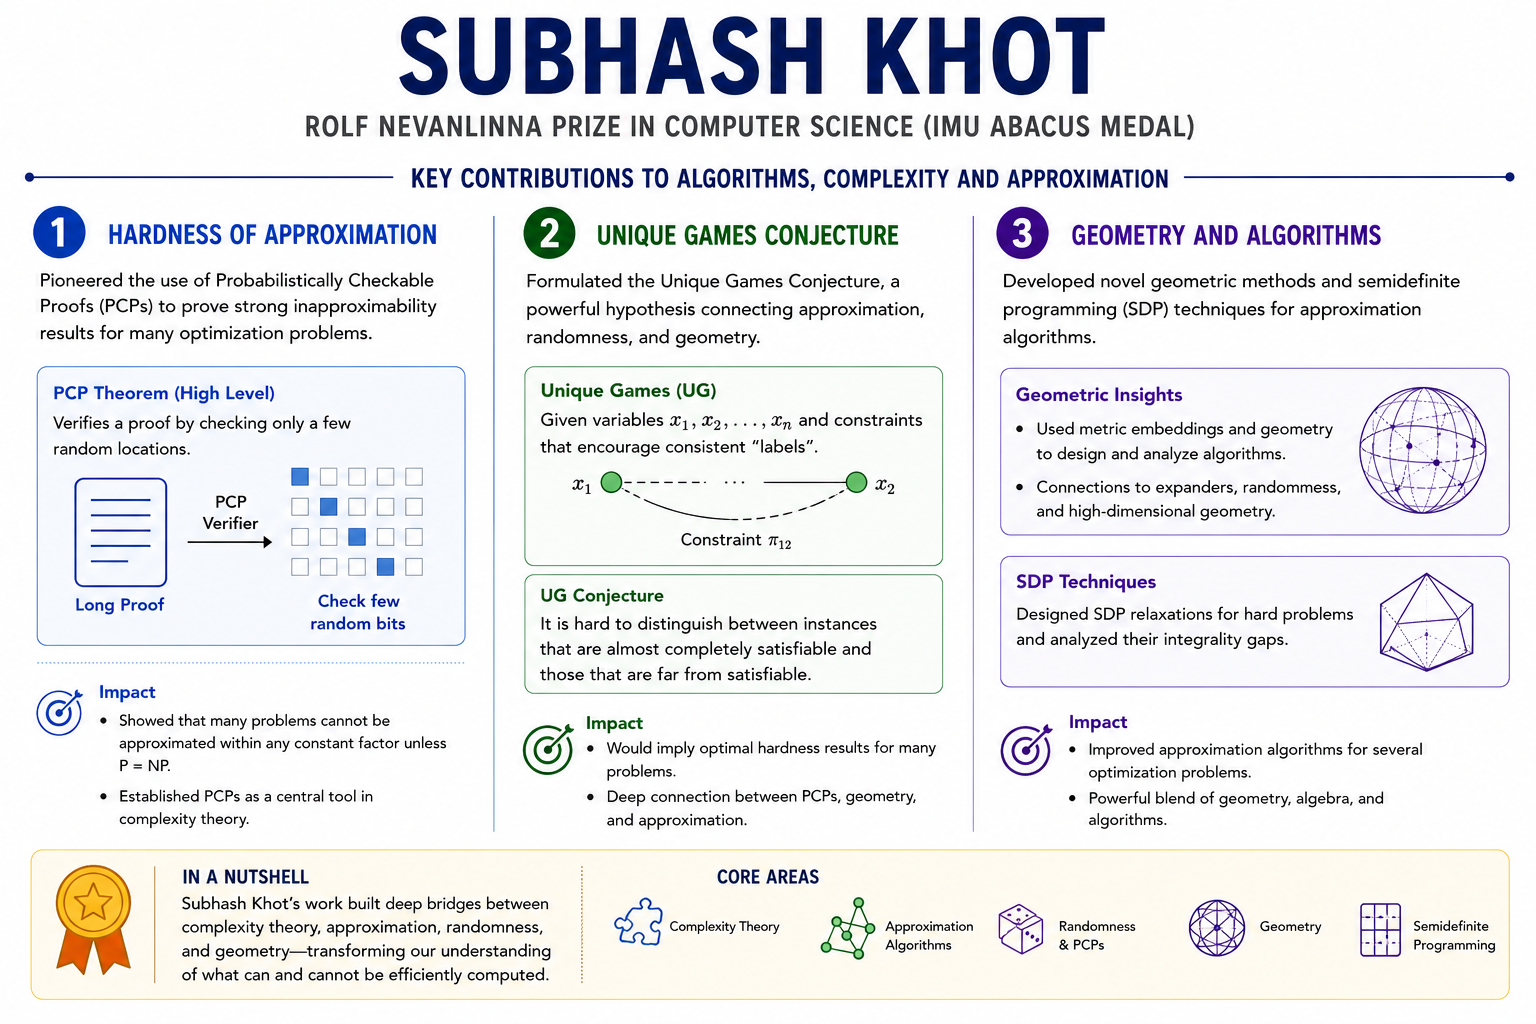
\includegraphics[width=\textwidth]{infographics/abacus9.png}
\end{center}
\targetchapterspacing
\index{Khot, Subhash}

\booknote{The central habit in this chapter is to judge a relaxation by its geometry: the angle between two vectors, not the list of labels, decides which approximation ratio is possible.}

\section{An Opening Story: A Party of Friends With Conflicting Labels}
Four friends---Ana, Bo, Cece, Di---wear tags labeled 0 or 1. Each friendship carries a rule: some pairs must match, others differ. Ana--Bo match, Bo--Cece differ, Cece--Di match, Di--Ana differ. Solution: Ana 0, Bo 0, Cece 1, Di 1.

Change one rule: Di--Ana must match. Walking around the circle forces Di's number to equal Ana's flipped, and to equal Ana's---impossible; the best is three of four rules, 75\%. A thousand friends and ten thousand rules behave the same at scale: each rule satisfiable alone, conflicts colliding around loops. Can a computer tell a party where nearly all rules hold from one where only a tiny fraction do? That question earned Subhash Khot the 2014 Rolf Nevanlinna Prize.

\section{The Problem}
NP-hard problems have no efficient exact algorithm (unless $\mathrm{P}=\mathrm{NP}$), so we accept approximations within a fixed ratio of optimal. Two questions: \emph{what ratio can an algorithm guarantee}, and \emph{what ratio can be proved impossible}? A factor of two may be easy while $1.01$ impossible---not for lack of cleverness but of proof: ruling out ratio $r$ needs instances where the optimum is high, every cheap method is trapped far below it, and a too-good algorithm would solve an NP-hard problem.

Such proofs used to be bespoke; the field wanted one ``mother'' constraint system whose hardness transfers everywhere, and an explanation of why thresholds land exactly where algorithms sit.

\section{The World Before}
\noindent\textbf{Exact optimization is NP-hard.} Since Cook's and Levin's theorems, no efficient exact algorithm exists for essentially every interesting optimization problem; the field retreated to approximation and to proving matching impossibility.

\noindent\textbf{Ratios, problem by problem.} By the early 1990s each problem had its own folklore: scattered, ad hoc proofs producing constants like 2, 1.5, and 0.5, with no unifying explanation.

\noindent\textbf{The PCP theorem.} In the mid-1990s it let every NP proof be checked by a verifier using logarithmically many random bits and querying only a constant number of proof bits; encoded as constraint systems, it became the first general hardness engine. H\aa stad showed MAX-3SAT cannot be beaten past $7/8$, matching the trivial random assignment, but each problem needed a new construction and the tools stalled on two-variable problems like MAX-CUT \cite{hastad-optimal}.

\noindent\textbf{An algorithm at 0.878.} Goemans and Williamson (1995) approximated MAX-CUT within $0.878$ via vectors and a random hyperplane. Unconditional PCP hardness reached only $16/17\approx0.941$; the matching $0.878+\eps$ was beyond the technology, and $0.878$ had no advance explanation \cite{goemans-williamson,hastad-optimal}.

\noindent\textbf{What was missing.} A single conjectured base problem whose hardness transfers everywhere, and a language in which the transfer is automatic. Khot supplied both; the base problem is Unique Games.

\section{The New Idea}
\subsection{A puzzle whose edges are permutations}
A \emph{unique game} is the party puzzle at scale. Vertices carry labels from $[k]$; each edge $(u,v)$ carries a bijection $\pi_e$ demanding $\pi_e(\text{label of }u)=\text{label of }v$. With two labels a permutation is just ``same'' or ``flip.'' Each constraint is one-to-one: fix one endpoint's label and the other's is forced. Every edge is locally trivial, so all difficulty is global, hidden in how permutations compose around cycles.

\subsection{The promise that makes it hard}
The Unique Games Conjecture (2002) concerns a \emph{promise problem}: the instance is either nearly perfect---at least $1-\delta$ of edges satisfiable---or almost empty---at most $\eps$---for tiny $\delta,\eps>0$. The conjecture: for every $\eps,\delta>0$ some label set size $k$ makes \emph{distinguishing the two cases NP-hard}. Fully satisfiable instances are easy on each connected component (guess one label per component and propagate); the difficulty is detecting global consistency when local demands never conflict \cite{khot-unique}.

\subsection{Why the seed is so powerful}
If problem $P$ reduces \emph{from} Unique Games, the promise survives: yes-instances become $P$-instances of value at least $c$, no-instances of value at most $s$. Any algorithm with approximation factor strictly better than $c/s$ would separate the cases. Because reductions are engineered outward from the game, $c/s$ can be tuned to targets like $0.878+\eps$: one hard promise, many exact thresholds.

\subsection{The geometry that fixes the threshold}
The companion tool is the \emph{semidefinite relaxation}. In the Boolean/MAX-CUT case, labels become unit vectors and constraints become angle statements. Rounding returns vectors to labels via a random hyperplane; an edge's survival probability depends only on the angle $\theta$ via $\theta/\pi$. For general Unique Games, the SDP instead uses vector variables for vertex-label pairs together with orthogonality and consistency constraints. The \emph{invariance principle}---high-dimensional discrete systems with no dominant variable behave like Gaussians---carries the game's discrete hardness into Gaussian geometry, where landmark thresholds can be computed exactly and matched to the best-known algorithms.

The conceptual shift: \emph{a single carefully designed constraint system can be the seed of hardness for many optimization problems; the geometry of the relaxation determines the threshold.}

\section{How It Works: Worked Examples}
\subsection{Two four-person parties, label by label}
Friends $A,B,C,D$; labels $\{0,1\}$; rules as equations $x_j=x_i\oplus b_{ij}$:
\begin{center}
\begin{tabular}{llc}
\toprule
Edge & Rule & Equation \\
\midrule
$(A,B)$ & same & $x_B=x_A$ \\
$(B,C)$ & flip & $x_C=x_B\oplus1$ \\
$(C,D)$ & same & $x_D=x_C$ \\
$(D,A)$ & flip & $x_A=x_D\oplus1$ \\
\bottomrule
\end{tabular}
\end{center}
Set $x_A=0$ and walk around: $x_B=0$, $x_C=1$, $x_D=1$, and the last rule needs $x_A=x_D\oplus1=0$---consistent. Two flips around the loop, and $0\oplus1\oplus1=0$; $(0,0,1,1)$ satisfies all four rules.

Instance 2: change the last rule to ``same,'' $x_A=x_D$. The walk gives $x_D=x_A\oplus1$, and the last rule demands $x_A=x_D=x_A\oplus1$---contradiction for either value of $x_A$. Each of the four assignments fails exactly one edge, so the best is $3/4=75\%$.

One flip instead of two. With two labels a cycle is fully satisfiable exactly when its flip count is even; with $k$ labels: \emph{the permutations around every cycle must compose to the identity}. Local constraints are individually satisfiable; only the product of permutations around closed walks decides global feasibility, and a label-recovery problem is hard precisely when this consistency is hard to detect.

\subsection{MAX-CUT: vectors, then a random wall between them}
MAX-CUT partitions a graph's vertices into two sides to maximize crossing edges---the two-label puzzle again, each edge demanding $x_u\ne x_v$.

The SDP relaxation assigns each vertex $i$ a unit vector $v_i$ and maximizes
\[
\sum_{(i,j)} \frac{1-v_i\cdot v_j}{2}.
\]
Rounding: pick a uniformly random direction $r$; put $i$ on the side $\operatorname{sign}(r\cdot v_i)$. Edge $(i,j)$ is cut when the signs disagree, with probability depending only on $\theta=\arccos(v_i\cdot v_j)$:
\[
\Pr[\text{cut}]=\frac{\theta}{\pi}.
\]
Three checks: $v_i\cdot v_j=0$ ($\theta=\pi/2$) gives $1/2$; $v_i=v_j$ ($\theta=0$) gives $0$; $v_i=-v_j$ ($\theta=\pi$) gives $1$.

At the worst angle, $\theta^*\approx0.74\pi$ (about $133^\circ$, $\cos\theta^*\approx-0.69$): the SDP contribution is $(1-(-0.69))/2\approx0.845$, but rounding cuts the edge with probability only $0.74$. The ratio $0.74/0.845\approx0.878$ is the minimum of $(\theta/\pi)\big/\big((1-\cos\theta)/2\big)$ over all angles---exactly the Goemans--Williamson factor. Their theorem: for \emph{every} graph, rounding any SDP solution cuts, in expectation, at least $0.878$ times the SDP value, hence $0.878$ times the optimum. Under Unique Games, beating $0.878+\eps$ is impossible (Khot, Kindler, Mossel, O'Donnell) \cite{goemans-williamson,khot-hardness}.

\section{The Mathematics in Brief}
\emph{The instance.} A Unique Game is a graph $(V,E)$ with label set $[k]$; each edge $e=(u,v)$ carries a bijection $\pi_e:[k]\to[k]$; an assignment $a$ satisfies $e$ when $\pi_e(a_u)=a_v$. Cycles are consistent exactly when their permutations compose to the identity.

\emph{The promise.} Distinguish $(1-\delta)$-satisfiable (some assignment satisfies $\ge1-\delta$ of the edges) from $\eps$-satisfiable (every assignment satisfies $\le\eps$). UGC: for every $\eps,\delta>0$ this is NP-hard for some label set size $k$.

\emph{The gap reduction.} If a reduction from Unique Games to $P$ preserves completeness $c$ and soundness $s$, no algorithm with approximation factor strictly better than $c/s$ can exist under UGC, or it would separate the cases.

\emph{MAX-CUT.} Relax to $\max\sum(1-v_i\cdot v_j)/2$ over unit vectors; round by a random hyperplane with $\Pr[\text{cut}]=\theta/\pi$. The inequality $\theta/\pi\ge\alpha(1-\cos\theta)/2$ with $\alpha\approx0.878567$ yields the approximation factor, and UGC-hardness rules out $\alpha+\eps$: the bounds meet.

\emph{The invariance principle.} A low-degree multilinear polynomial of many weakly correlated discrete variables with no dominant variable is distributed nearly like the same polynomial on Gaussians with matching correlations---many small independent contributions converge to a Gaussian. It moves hardness from discrete games into Gaussian space, where isoperimetric theorems can compute sharp thresholds.

\section{Limits and Modern Views}
\emph{A conjecture, not a theorem.} UGC remains open, so results conditional on it must be labeled as such; some stronger formulations were disproved. The neighbouring \emph{2-to-2 Games Conjecture} (constraints two-to-two instead of one-to-one) was completed in 2018 in an imperfect-completeness form through work by Khot, Minzer, and Safra, building on the reduction and framework of Dinur, Khot, Kindler, Minzer, and Safra. It yields unconditional hardness results for vertex cover approaching $\sqrt2$ (beyond the long-standing $1.36$ bound) and for independent set, and strengthens belief in UGC \cite{dkkms-2to2,kms-2to2}. Specialized families are understood; the general promise is not.

\emph{Unconditional gaps are weaker.} An integrality gap shows one relaxation cannot certify a better ratio; it says nothing about stronger algorithms, while UGC hardness would settle the question.

\emph{Structure beats worst cases.} Hardness is worst-case; sparse graphs, clustered data, and inputs with known distributions carry structure algorithms exploit. The right response to a barrier is diagnosis: ask what the fractional solution knows, what the integral solution requires, and which correlation the rounding step forgot.

\emph{Where the field went.} Sum-of-squares hierarchies seek stronger relaxations; spectral and local algorithms exploit expansion; and, assuming UGC, Raghavendra showed that the best polynomial-time ratio for every constraint satisfaction problem is characterized by the geometry of a suitable SDP relaxation \cite{raghavendra-csp}.

\section{Exercises and Self-Study Guide}
\begin{enumerate}[label=\textbf{E\arabic*.}]
\item Verify both party instances by writing out all four assignments; then build a five-vertex cycle with exactly two flips and show it is fully satisfiable.
\hint{A two-label cycle is satisfiable exactly when its flip count is even; fix one label and propagate.}
\item Explain how the promise---``$(1-\delta)$- or $\eps$-satisfiable''---differs from ``is this instance fully satisfiable?'', and why the latter is easy.
\hint{A promise problem answers only on the two guaranteed input kinds; a fully satisfiable unique game is solved by propagating one guessed label.}
\item For vectors with $v_i\cdot v_j=1/2$ and $v_i\cdot v_j=-1/2$, compute the angle $\theta$, the SDP contribution $(1-v_i\cdot v_j)/2$, and the cut probability $\theta/\pi$. Which angle loses more?
\hint{$\arccos(1/2)=\pi/3$: cut probability $1/3$, contribution $1/4$, ratio $4/3$; only near $\theta^*\approx0.74\pi$ does the ratio fall to $0.878$.}
\item A gap reduction has completeness $c=0.9$ and soundness $s=0.3$. If an algorithm returns at least $\mathrm{OPT}/r$, which $r$ separate yes from no by output size?
\hint{Separation needs $0.9/r>0.3$, so $r<3$; in general the factor ruled out is $c/s$.}
\item Identify a global property of the party cycle that a local pairwise relaxation cannot express.
\hint{Each flip is locally satisfiable by half of all label pairs; only the product of permutations around a loop records feasibility.}
\item Build a tiny integer program whose relaxation beats the integral optimum: cover the triangle, $x_A+x_B\ge1$, $x_B+x_C\ge1$, $x_A+x_C\ge1$, minimize the sum, $x_i\in\{0,1\}$.
\hint{$(1/2,1/2,1/2)$ costs $1.5$; every integral cover costs $2$.}
\item Give a rounding rule that preserves every marginal but violates a pairwise ``must be equal'' constraint with positive probability.
\hint{Independent rounding to 0 with probability $p$: marginals match, but two forced-equal variables agree only with probability $p^2+(1-p)^2$.}
\end{enumerate}

\booknote{A final exercise in judgment: whenever a relaxation seems to declare a problem easy, ask what the fractional solution knows, what the integral solution requires, and which correlation the rounding step forgot.}
\clearpage
